\documentclass{beamer}
\usetheme{Boadilla}

\makeatother
\setbeamertemplate{footline}
{
    \leavevmode%
    \hbox{%
    \begin{beamercolorbox}[wd=.4\paperwidth,ht=2.25ex,dp=1ex,center]{author in head/foot}%
        \usebeamerfont{author in head/foot}\insertshortauthor
    \end{beamercolorbox}%
    \begin{beamercolorbox}[wd=.55\paperwidth,ht=2.25ex,dp=1ex,center]{title in head/foot}%
        \usebeamerfont{title in head/foot}\insertshorttitle
    \end{beamercolorbox}%
    \begin{beamercolorbox}[wd=.05\paperwidth,ht=2.25ex,dp=1ex,center]{date in head/foot}%
        \insertframenumber{}
    \end{beamercolorbox}}%
    \vskip0pt%
}
\makeatletter
\setbeamertemplate{navigation symbols}{}

\usepackage[T1]{fontenc}
\usepackage{lmodern}
\usepackage{amssymb,amsmath}
\renewcommand{\familydefault}{\sfdefault}

\DeclareMathOperator*{\argmax}{argmax}

\usepackage{mathtools}
\usepackage{graphicx}
\usepackage{threeparttable}
\usepackage{booktabs}
\usepackage{siunitx}
\sisetup{parse-numbers=false}

%\setlength{\OuterFrameSep}{-2pt}
%\makeatletter
%\preto{\@verbatim}{\topsep=-10pt \partopsep=-10pt }
%\makeatother

\title[Lecture 25:\ Endogeneity III]{Lecture 25:\ Endogeneity III}
\author[ResEcon 703:\ Advanced Econometrics]{ResEcon 703:\ Topics in Advanced Econometrics}
\date{Matt Woerman\\University of Massachusetts Amherst}

\begin{document}

{\setbeamertemplate{footline}{} 
\begin{frame}[noframenumbering]
    \titlepage
\end{frame}
}

\begin{frame}\frametitle{Agenda}
    Last time
    \begin{itemize}
        \item Berry, Levinsohn, and Pakes (1995)
    \end{itemize}
    \vspace{2ex}
    Today
    \begin{itemize}
        \item Berry, Levinsohn, and Pakes (1995)
    \end{itemize}
    \vspace{2ex}
    Upcoming
    \begin{itemize}
        \item Final exam
        \begin{itemize}
        	\item Final exam is posted, due December 19
        \end{itemize}
        \item Course surveys
        \begin{itemize}
            \item Course surveys are open, due December 22
            \item \href{http://owl.umass.edu/partners/courseEvalSurvey/uma/}{Click here (\texttt{owl.umass.edu/partners/courseEvalSurvey/uma})}
        \end{itemize}
    \end{itemize}
\end{frame}

\begin{frame}\frametitle{}
    \vfill
    \centering
    \begin{beamercolorbox}[center]{title}
        \Large Berry, Levinsohn, and Pakes (1995)
    \end{beamercolorbox}
    \vfill
\end{frame}

\begin{frame}\frametitle{Summary of BLP Theoretical Models}
    BLP develop models of demand and supply
    \begin{itemize}
        \item Random coefficients model of demand for differentiated products
        \item Nash-Bertrand pricing model with oligopolistic competition
    \end{itemize}
    \vspace{2ex}
    Both of these models suffer from endogeneity
    \begin{itemize}
        \item BLP need instruments to recover unbiased parameter estimates
    \end{itemize}
    \vspace{2ex}
    The endogeneity enters these models nonlinearly
    \begin{itemize}
        \item BLP develop a new estimation method to handle instruments in a nonlinear model
    \end{itemize}
\end{frame}

\begin{frame}\frametitle{Instruments}
    BLP need to find instruments for both the demand equation and the pricing equation \\
    \vspace{2ex}
    Appropriate instruments must satisfy two conditions
    \begin{itemize}
        \item Correlated with observed product attributes, $x_{jt}$, and cost characteristics, $w_{jt}$
        \item Not correlated with unobserved utility, $\xi_{jt}$, or unobserved marginal costs, $\omega_{jt}$
    \end{itemize}
    \vspace{2ex}
    BLP construct instruments from the attributes and cost characteristics of all products
    \begin{itemize}
        \item The justification for these instruments comes from a mean independence assumption
    \end{itemize}
\end{frame}

\begin{frame}\frametitle{Mean Independence Assumption}
    BLP assume that unobserved utility, $\xi_{jt}$, and unobserved marginal costs, $\omega_{jt}$, for each product is mean independent of all product attributes and cost characteristics
    \begin{align*}
        0 &= E(\xi_{jt} \mid z_t) = E(\omega_{jt} \mid z_t) \\
        \intertext{where}
        z_{jt} &= (x_{jt}, w_{jt}) \\
        z_t &= (z_{1t}, \ldots, z_{Jt})
    \end{align*} \\
    \vspace{2ex}
    In other words, observed product attributes and cost characteristics are exogenously (or at least previously) determined, and the unobserved utility and marginal costs are effectively random noise
    \begin{itemize}
        \item But what if all product attributes are jointly determined?
    \end{itemize}
\end{frame}

\begin{frame}\frametitle{BLP Instruments}
    BLP argue there are three first-order instruments for each product attribute or cost characteristic
    \begin{itemize}
        \item The attribute (cost characteristic) itself
        \item The sum of the attribute (cost characteristic) for the firm's other products
        \item The sum of the attribute (cost characteristic) for the products produced by other firms
    \end{itemize}
    \vspace{2ex}
    They provide some intuition for these instruments, as well as a more formal proof
    \begin{itemize}
        \item Products that face good substitutes tend to have low markups, and products without good substitutes tend to have higher markups
        \item Markups will respond differently to own and rival products
    \end{itemize}
    \vspace{2ex}
    This argument relies on the exogeneity of attributes in the product space
\end{frame}

\begin{frame}\frametitle{BLP Estimation}
    The intuition of the BLP estimation strategy is relatively simple, but practically implementing it is more complex
    \begin{itemize}
        \item Given data on prices and other product attributes, any set of
        \begin{enumerate}
            \item Observed market shares, $S$
            \item Demand model parameters, $\theta_1$
            \item Parameters relating to consumer characteristics, $\theta_2$
            \item Cost function parameters, $\gamma$
        \end{enumerate}
        \item[] yields a unique set of unobserved utilities, $\xi_{jt}(x_t, p_t, S_t; \theta_1, \theta_2)$, and unobserved marginal costs, $\omega_{jt}(x_t, p_t, w_{jt}, S_t; \theta_2, \gamma)$
        \item Assuming we can compute these values, $\xi_{jt}(x_t, p_t, S_t; \theta_1, \theta_2)$ and $\omega_{jt}(x_t, p_t, w_{jt}, S_t; \theta_2, \gamma)$ are uncorrelated with the instruments at the true parameter values
        \item Use MSM to find the set of parameters that results in no (or minimal) correlation between $\xi_{jt}(x_t, p_t, S_t; \theta_1, \theta_2)$ and $\omega_{jt}(x_t, p_t, w_{jt}, S_t; \theta_2, \gamma)$ and the instruments
    \end{itemize}
    \vspace{1ex}
    But computing $\xi_{jt}(x_t, p_t, S_t; \theta_1, \theta_2)$ and $\omega_{jt}(x_t, p_t, w_{jt}, S_t; \theta_2, \gamma)$ is difficult!
\end{frame}

\begin{frame}\frametitle{BLP Estimation Steps}
    BLP use MSM to loop over parameters, $\theta$, and converge to the set of $\hat{\theta}$ that minimize the MSM objective function, and each loop requires four steps that depend on $\theta$
    \begin{enumerate}
        \item Invert the estimation of market shares, $s_{jt}(x_t, p_t, \delta_t; \theta_2)$, to get estimates of $\delta_{jt}(x_t, p_t, S_t; \theta_2)$
        \item Solve for the vector of unobserved utilities, $\xi_{jt}(x_t, p_t, S_t; \theta_1, \theta_2)$, implied by $\delta_{jt}(x_t, p_t, S_t; \theta_2)$ and other demand model parameters, $\theta_1$
        \item Calculate the vector of unobservable marginal costs, $\omega_{jt}(x_t, p_t, w_{jt}, S_t; \theta_2, \gamma)$, implied by markups, $b_{jt}(x_t, p_t, \delta_t; \theta_2)$, and cost function parameters, $\gamma$
        \item Calculate all 34 (!) empirical moments, $G(\theta; x, p, w, S)$
        \begin{itemize}
            \item Product of $\xi_{jt}(x_t, p_t, S_t; \theta_1, \theta_2)$ and 15 demand instruments
            \item Product of $\omega_{jt}(x_t, p_t, w_{jt}, S_t; \theta_2, \gamma)$ and 19 cost instruments
        \end{itemize}
    \end{enumerate}
\end{frame}

\begin{frame}\frametitle{BLP Estimation with Logit Assumptions}
    BLP first estimate their model with the logit assumptions
    \begin{itemize}
        \item $\mu_{ijt} = 0$: no individual-specific utility from observable attributes
        \item $\varepsilon_{ijt} \sim$ i.i.d.\ type I extreme value
    \end{itemize}
    \vspace{3ex}
    Estimation with logit assumptions serves two purposes
    \begin{itemize}
        \item Provides a benchmark to compare their random coefficient estimates to demonstrate what is gained by their innovative approach
        \item Eases the reader into an easier estimation procedure
    \end{itemize}
\end{frame}

\begin{frame}\frametitle{BLP Logit Model: Step 1}
    With the logit assumptions, the utility model simplifies to 
    \begin{align*}
        u_{ijt} &= \delta_{jt}(x_{jt}, p_{jt}, \xi_{jt}; \theta_1) + \varepsilon_{ijt} \\
        \intertext{where}
        \delta_{jt}(x_{jt}, p_{jt}, \xi_{jt}; \theta_1) &= x_{jt} \beta - \alpha p_{jt} + \xi_{jt}
    \end{align*} \\
    \vspace{2ex}
    Then market shares are simply
    $$s_{jt}(x_t, p_t, \delta_t) = \frac{e^{\delta_{jt}}}{1 + \sum_{\ell = 1}^{J_t} e^{\delta_{\ell t}}}$$
    which is easily inverted to estimate $\delta_{jt}$ using observed market shares
    $$\delta_{jt}(S_t) = \ln(S_{jt}) - \ln(S_{0t})$$
\end{frame}

\begin{frame}\frametitle{BLP Logit Model: Steps 2--4}
    Step 2: The vector of unobserved utilities is easily calculated as
    \begin{align*}
        \xi_{jt}(x_t, p_t, S_t; \theta_1) &= \delta_{jt}(S_t) - x_{jt} \beta + \alpha p_{jt} \\
        &=  \ln(S_{jt}) - \ln(S_{0t}) - x_{jt} \beta + \alpha p_{jt}
    \end{align*} \\
    \vspace{1ex}
    Step 3: The calculation of $\omega_{jt}(x_t, p_t, w_{jt}, S_t; \gamma)$ is also straightforward \\
    \vspace{2ex}
    Step 4: Empirical moments are calculated as
    $$G(\theta; x, p, w, S) = \frac{1}{\sum_{t = 1}^T J_t} \sum_{t = 1}^T \sum_{j = 1}^{J_t} H_{jt}(z_t) 
    \begin{pmatrix}
        \xi_{jt}(x_t, p_t, S_t; \theta_1) \\
        \omega_{jt}(x_t, p_t, w_{jt}, S_t; \gamma)
    \end{pmatrix}$$
    where $H_{jt}(z_t)$ is the matrix of instruments for product $j$ in market $t$ \\
    \vspace{2ex}
    BLP uses GMM to find the set of parameters $\hat{\theta}$ that minimizes these empirical moments
\end{frame}

\begin{frame}\frametitle{BLP Estimation with Mixed Logit Assumptions}
    The full BLP model uses the less restrictive assumptions of the mixed logit model
    \begin{itemize}
        \item These assumptions yield more realistic substitution patterns between automobiles
        \item They also make the estimation much more difficult
    \end{itemize}
    \vspace{2ex}
    What makes it so difficult?
    \begin{itemize}
        \item Steps 1 and 3 no longer have closed-form expressions and require simulation
        \item The inversion in step 1 is computationally infeasible using traditional (at the time) estimation methods
    \end{itemize}
    \vspace{2ex}
    BLP must develop their own estimation method
\end{frame}

\begin{frame}\frametitle{BLP Mixed Logit Model: Step 1}
    With the mixed logit assumptions, market shares are
    \begin{align*}
        s_{jt}(x_t, p_t, \delta_t; \theta_2) &= \int L_{ijt}(x_t, p_t, \delta_t, \nu_i, D_i; \theta_2) dP_{\nu}^*(\nu) d\hat{P}_D^*(D) \\
        \intertext{where}
        L_{ijt}(x_t, p_t, \delta_t, \nu_i, D_i; \theta_2) &= \frac{e^{\delta_{jt} + \mu_{ijt}(x_{jt}, p_{jt}, \nu_i, D_i; \theta_2)}}{1 + \sum_{\ell = 1}^{J_t} e^{\delta_{\ell t} + \mu_{i \ell t}(x_{\ell t}, p_{\ell t}, \nu_i, D_i; \theta_2)}} \\
        \intertext{These market shares can be simulated as}
        \check{s}_{jt}(x_t, p_t, \delta_t; \theta_2) &= \frac{1}{R} \sum_{i = 1}^R \frac{e^{\delta_{jt} + \mu_{ijt}(x_{jt}, p_{jt}, \nu_i, D_i; \theta_2)}}{1 + \sum_{\ell = 1}^{J_t} e^{\delta_{\ell t} + \mu_{i \ell t}(x_{\ell t}, p_{\ell t}, \nu_i, D_i; \theta_2)}}
    \end{align*}
    where each $\nu_i$ and $D_i$ is drawn from $P_{\nu}^*(\nu)$ and $\hat{P}_D^*(D)$, respectively
\end{frame}

\begin{frame}\frametitle{BLP Contraction Mapping}
    BLP could theoretically estimate the vector of unobserved utilities, $\delta_{jt}(x_t, p_t, S_t; \theta_2)$, by iterating through possible vectors and finding one that yields the observed market shares
    \begin{itemize}
        \item But this is computationally infeasible!
    \end{itemize}
    \vspace{2ex}
    Instead, BLP prove there is a contraction mapping between market shares and $\delta_{jt}(x_t, p_t, S_t; \theta_2)$
    \begin{itemize}
        \item Every possible vector of market shares yields a unique vector of $\delta_{jt}(x_t, p_t, S_t; \theta_2)$
        \item An iterative algorithm will converge to this unique vector of $\delta_{jt}(x_t, p_t, S_t; \theta_2)$
    \end{itemize}
    \vspace{2ex}
    $$\delta_t^{h+1} = \delta_t^h + \ln(S_t) - \ln(\check{s}_{jt}(x_t, p_t, \delta_t^h; \theta_2))$$
    with $\check{s}_{jt}(x_t, p_t, \delta_t^h; \theta_2)$ simulated as on the previous slide
\end{frame}

\begin{frame}\frametitle{BLP Mixed Logit Model: Steps 2--4}
    Step 2: The vector of unobserved utilities is easily calculated as
    $$\xi_{jt}(x_t, p_t, S_t; \theta_1, \theta_2) = \delta_{jt}(x_t, p_t, S_t; \theta_2) - x_{jt} \beta + \alpha p_{jt}$$ \\
    \vspace{1ex}
    Step 3: The calculation of $\omega_{jt}(x_t, p_t, w_{jt}, S_t; \gamma)$ requires simulation, which is not trivial but also not particularly innovative
    \begin{itemize}
        \item See the paper for more details
    \end{itemize}
    \vspace{2ex}
    Step 4: Empirical moments are calculated as
    $$G(\theta; x, p, w, S) = \frac{1}{\sum_{t = 1}^T J_t} \sum_{t = 1}^T \sum_{j = 1}^{J_t} H_{jt}(z_t) 
    \begin{pmatrix}
        \xi_{jt}(x_t, p_t, S_t; \theta_1) \\
        \omega_{jt}(x_t, p_t, w_{jt}, S_t; \gamma)
    \end{pmatrix}$$
    where $H_{jt}(z_t)$ is the matrix of instruments for product $j$ in market $t$ \\
    \vspace{2ex}
    BLP uses MSM to find the set of parameters $\hat{\theta}$ that minimizes these empirical moments
\end{frame}

\begin{frame}\frametitle{Data}
    BLP use data on cars sold in the US in the years 1971 to 1990
    \begin{itemize}
        \item 20 years of data with 2217 total model-years
        \item 997 distinct models once similar model-years are aggregated
    \end{itemize}
    \vspace{2ex}
    Variables in each model \\
    \begin{columns}
        \begin{column}{0.5\textwidth}
            \begin{itemize}
                \item Demand model
                \begin{itemize}
                    \item Constant
                    \item Horsepower / weight
                    \item Air conditioning
                    \item Miles per dollar
                    \item Size
                    \item Price
                \end{itemize}
            \end{itemize}
        \end{column}
        \begin{column}{0.5\textwidth}
            \begin{itemize}
                \item Supply model
                \begin{itemize}
                    \item Constant
                    \item Horsepower / weight
                    \item Air conditioning
                    \item Miles per gallon
                    \item Size
                    \item Trend
                \end{itemize}
            \end{itemize}
        \end{column}
    \end{columns}
\end{frame}

\begin{frame}\frametitle{Estimation Results}
    \begin{columns}
        \begin{column}{0.4\textwidth}
            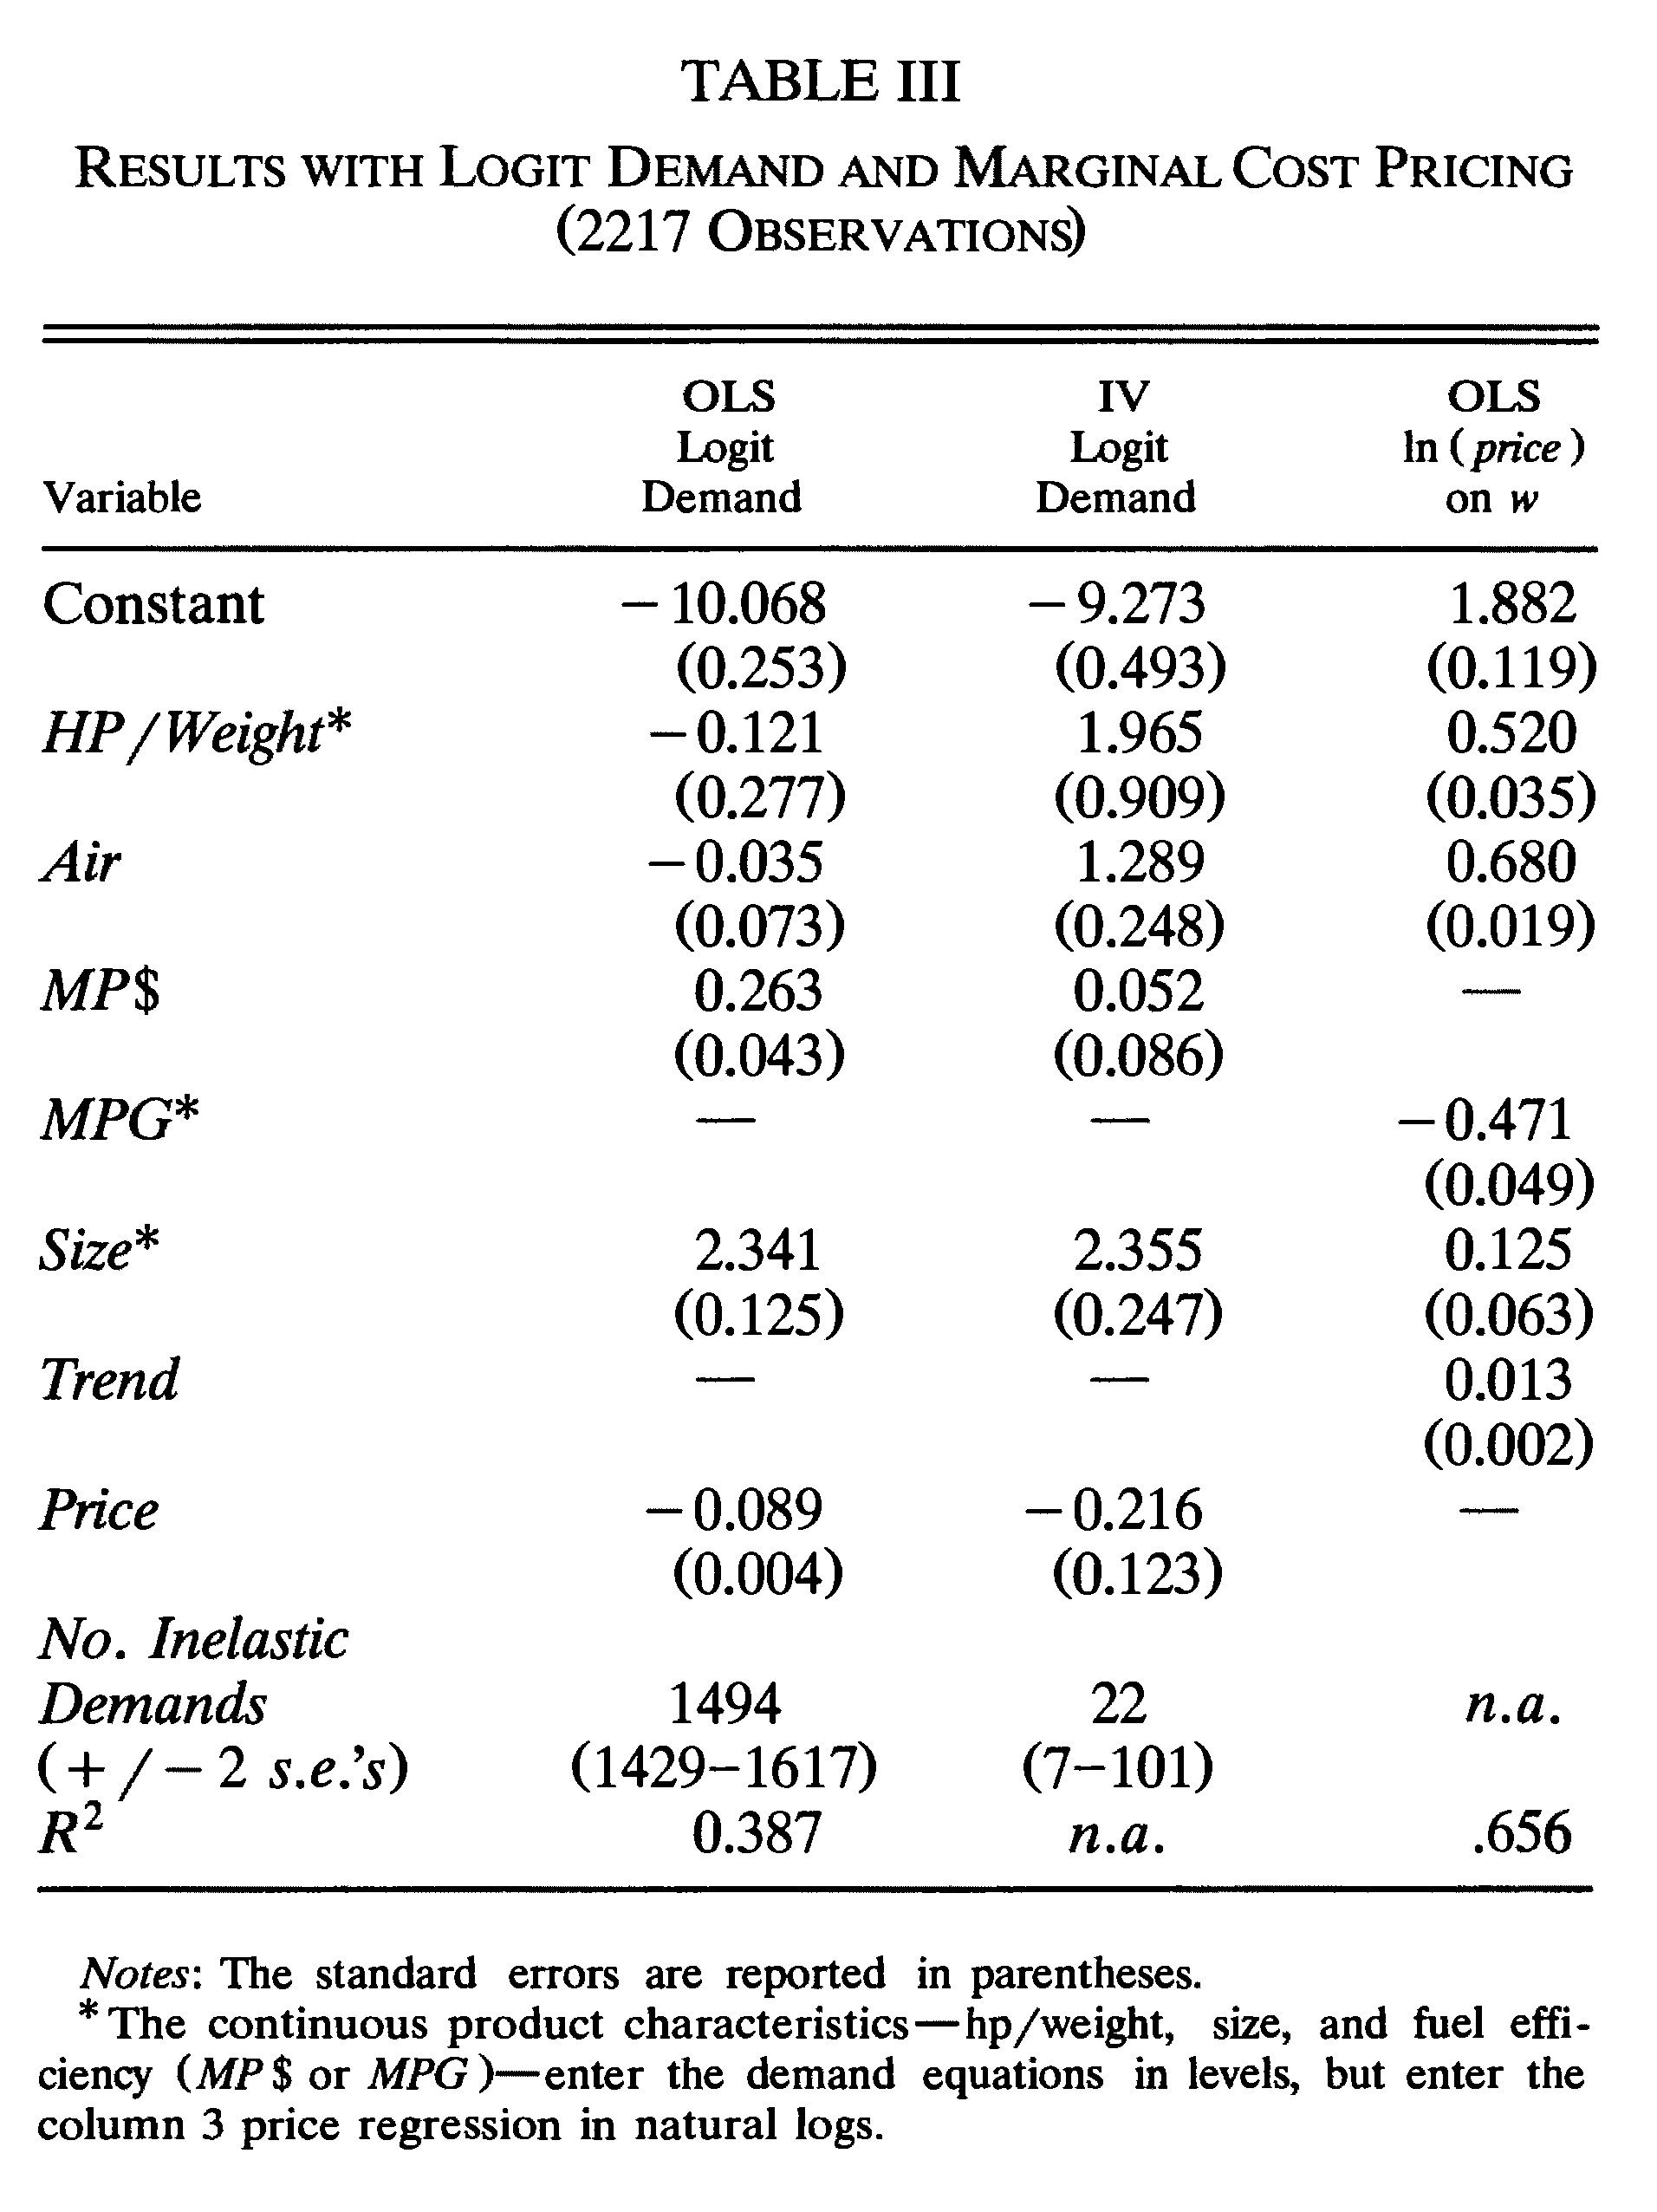
\includegraphics[width=\textwidth]{logit_results.png}
        \end{column}
        \begin{column}{0.6\textwidth}
            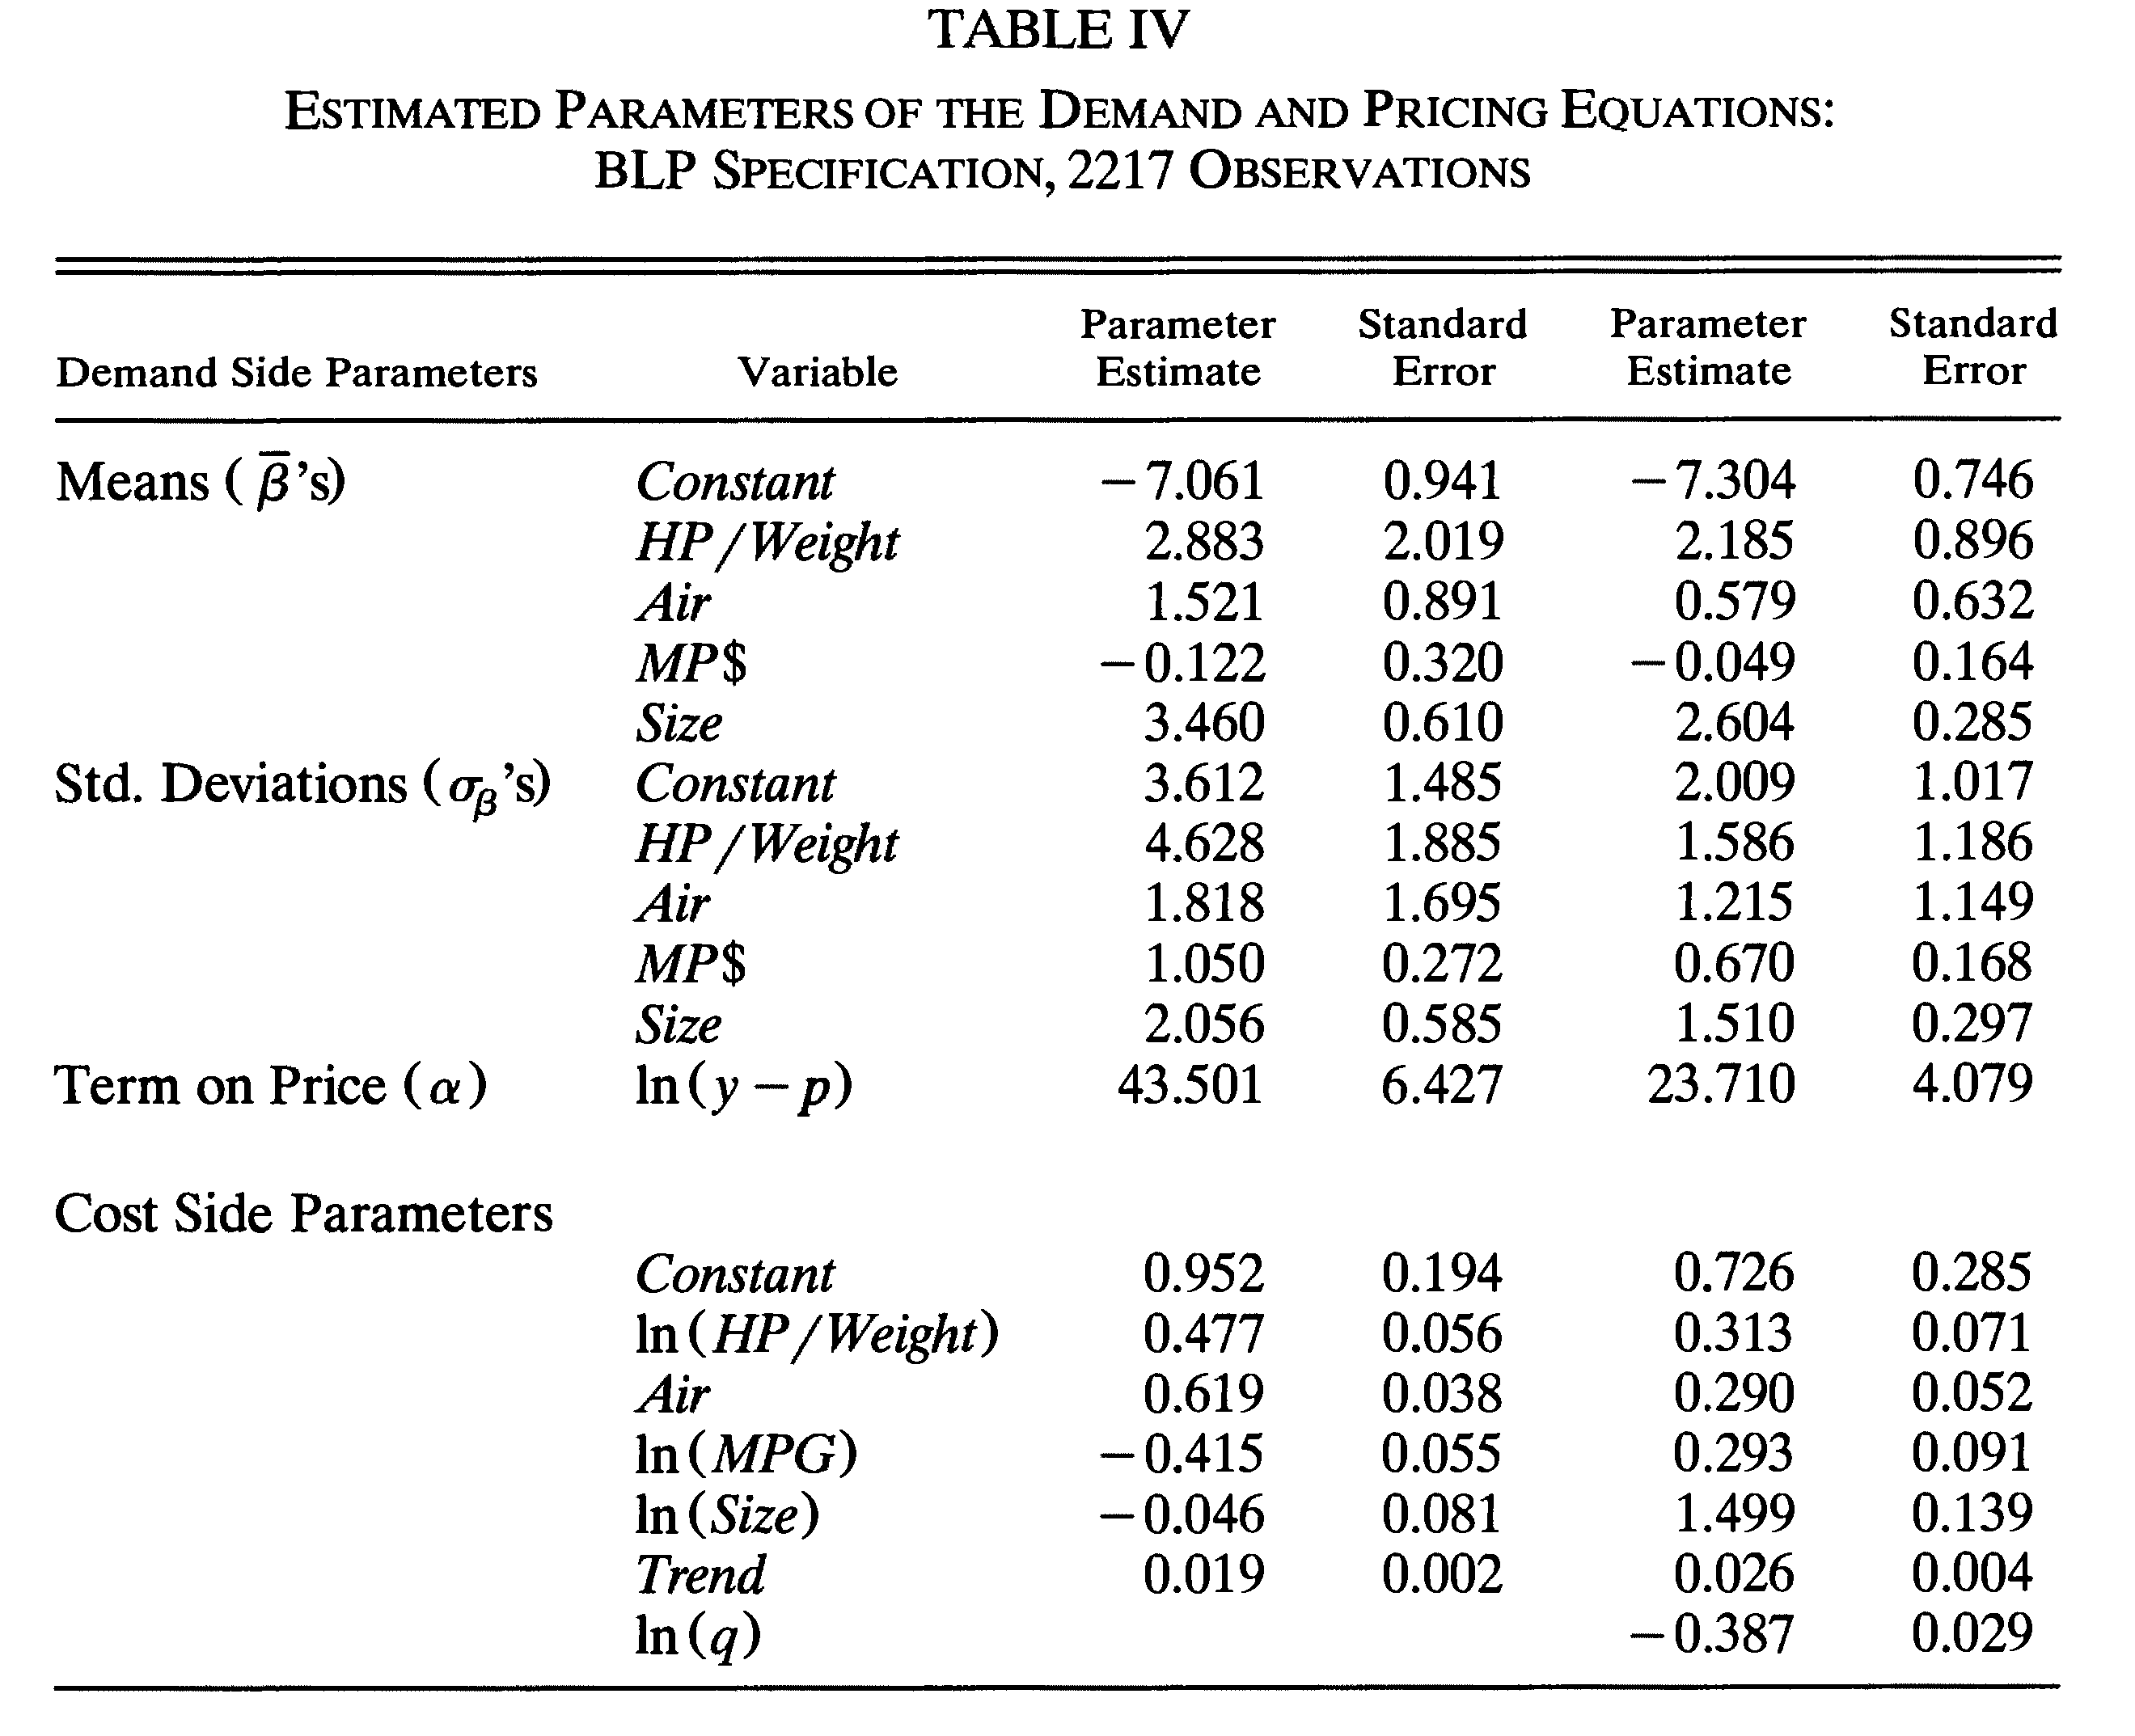
\includegraphics[width=\textwidth]{mixed_logit_results.png}
        \end{column}
    \end{columns}
\end{frame}

\begin{frame}\frametitle{Attribute Elasticities}
    \centering
    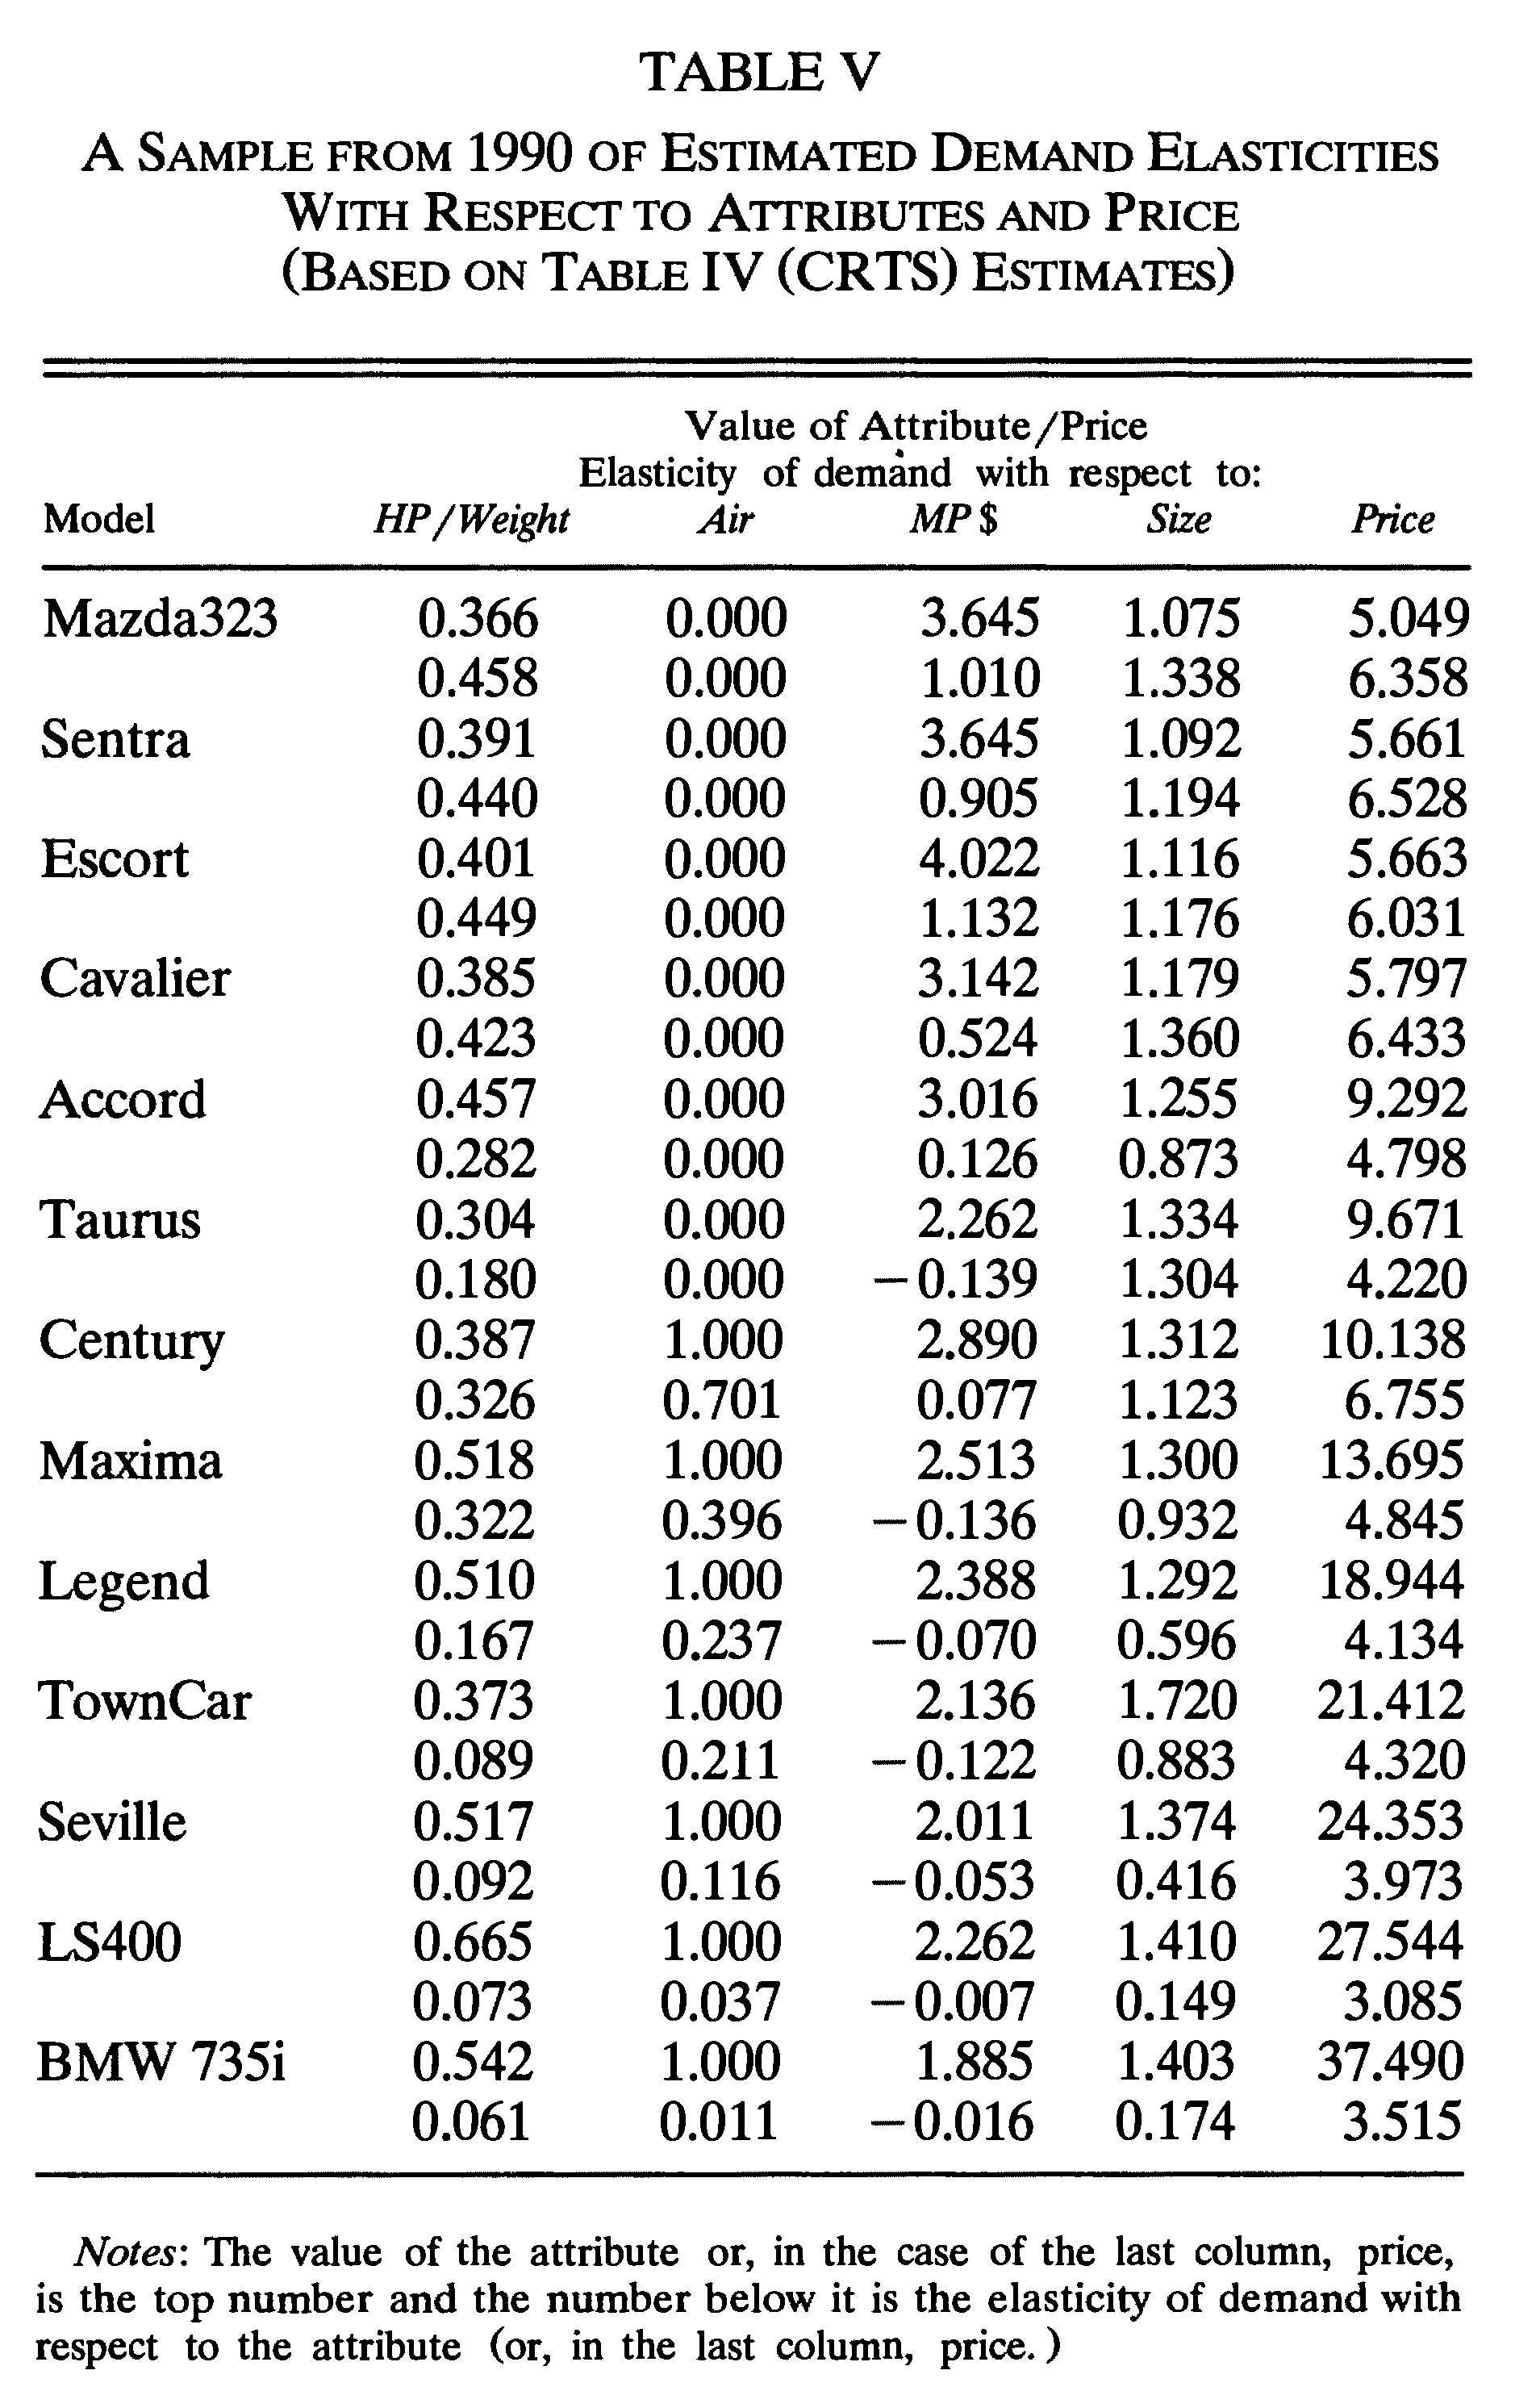
\includegraphics[width=0.43\textwidth]{attribute_elasticities.png}
\end{frame}

\begin{frame}\frametitle{Price Elasticities}
    \centering
    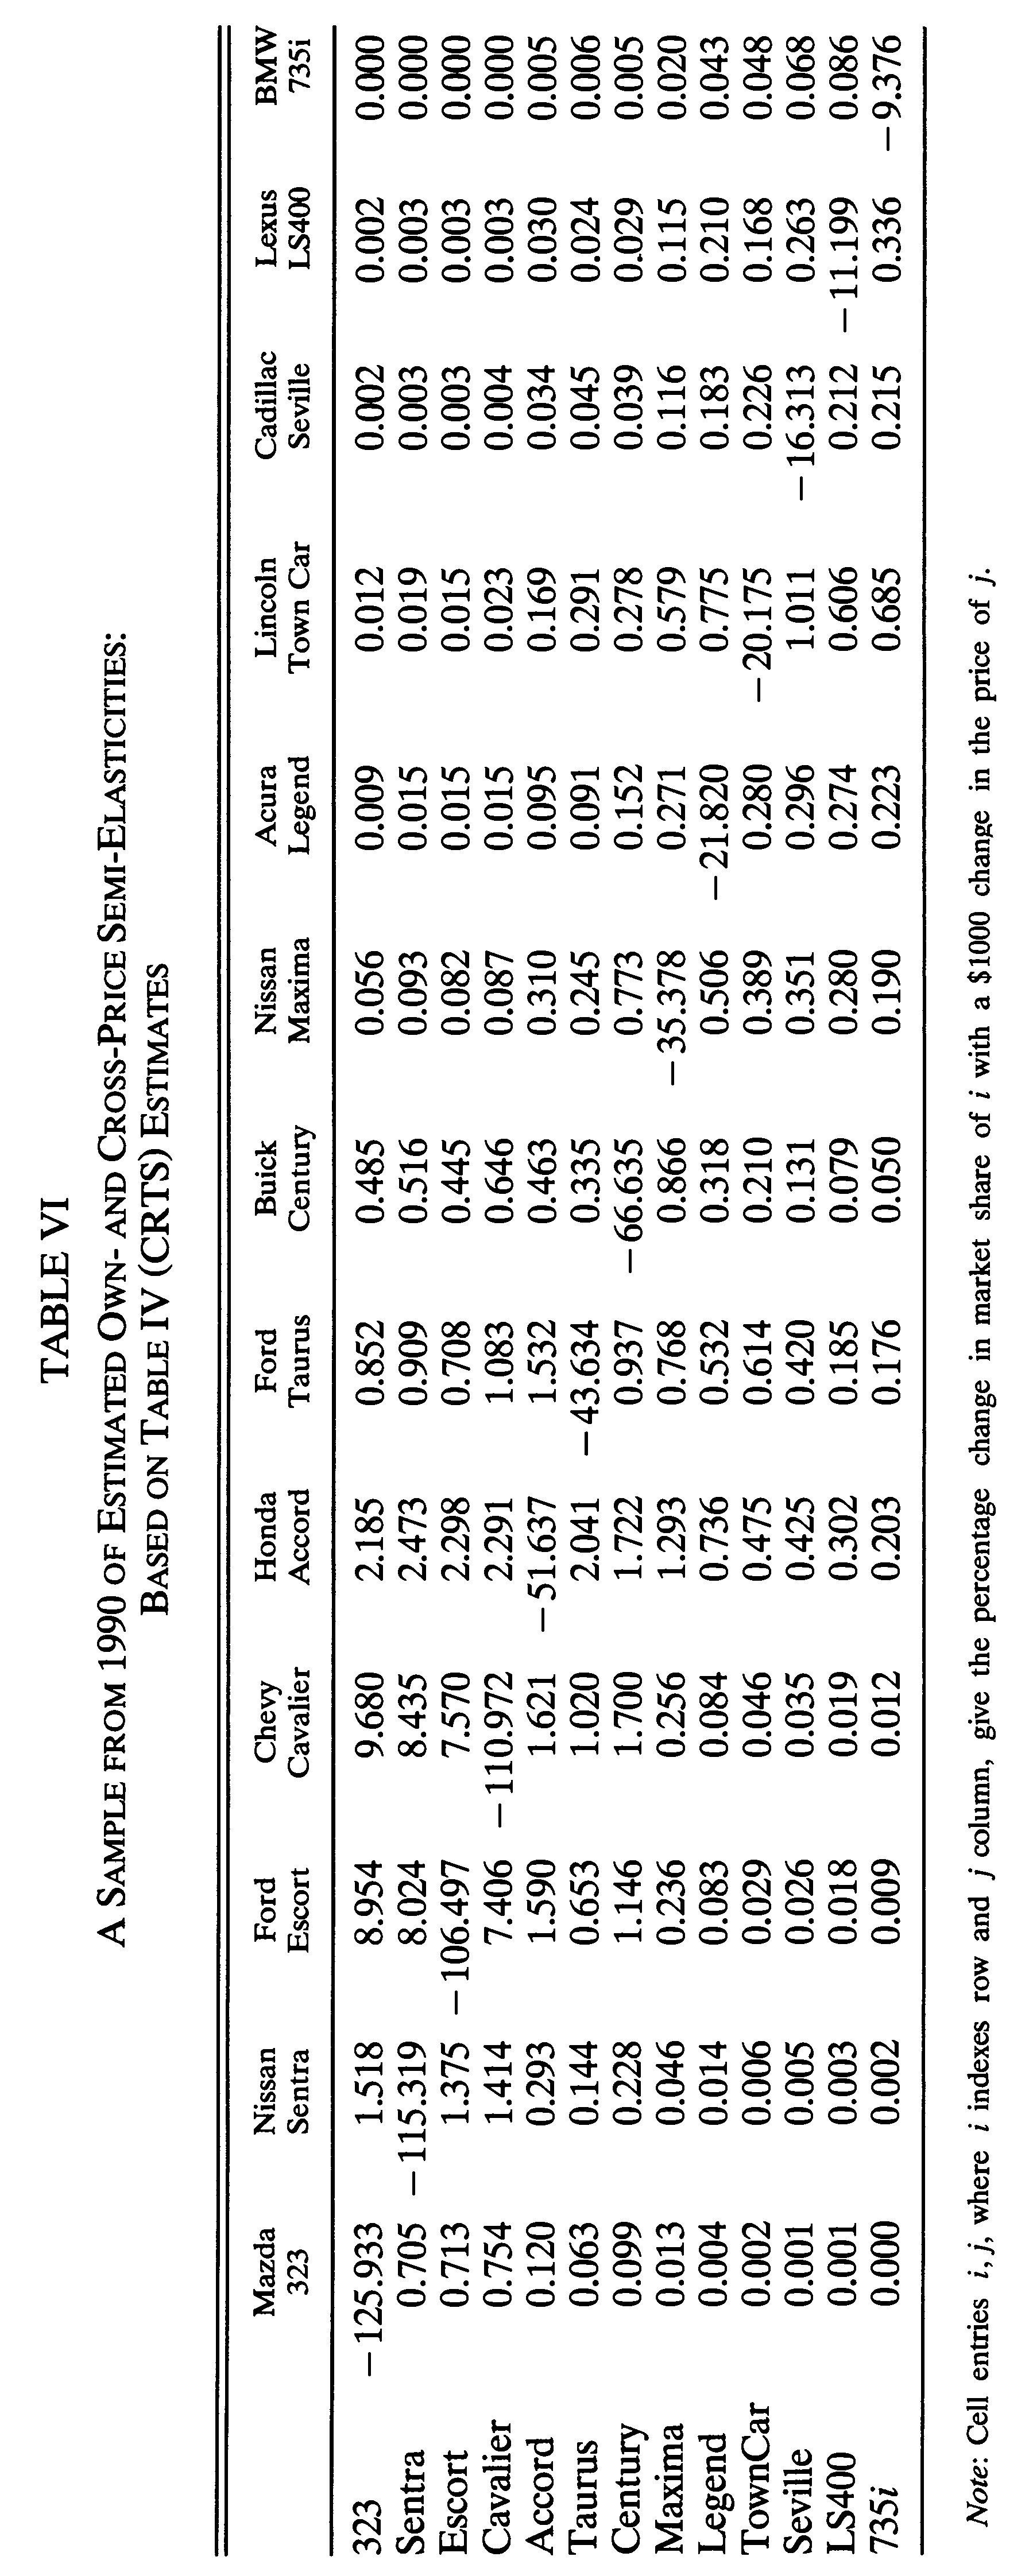
\includegraphics[angle=270, width=\textwidth]{price_elasticities.png}
\end{frame}

\begin{frame}\frametitle{Substitution to the Outside Good}
    \centering
    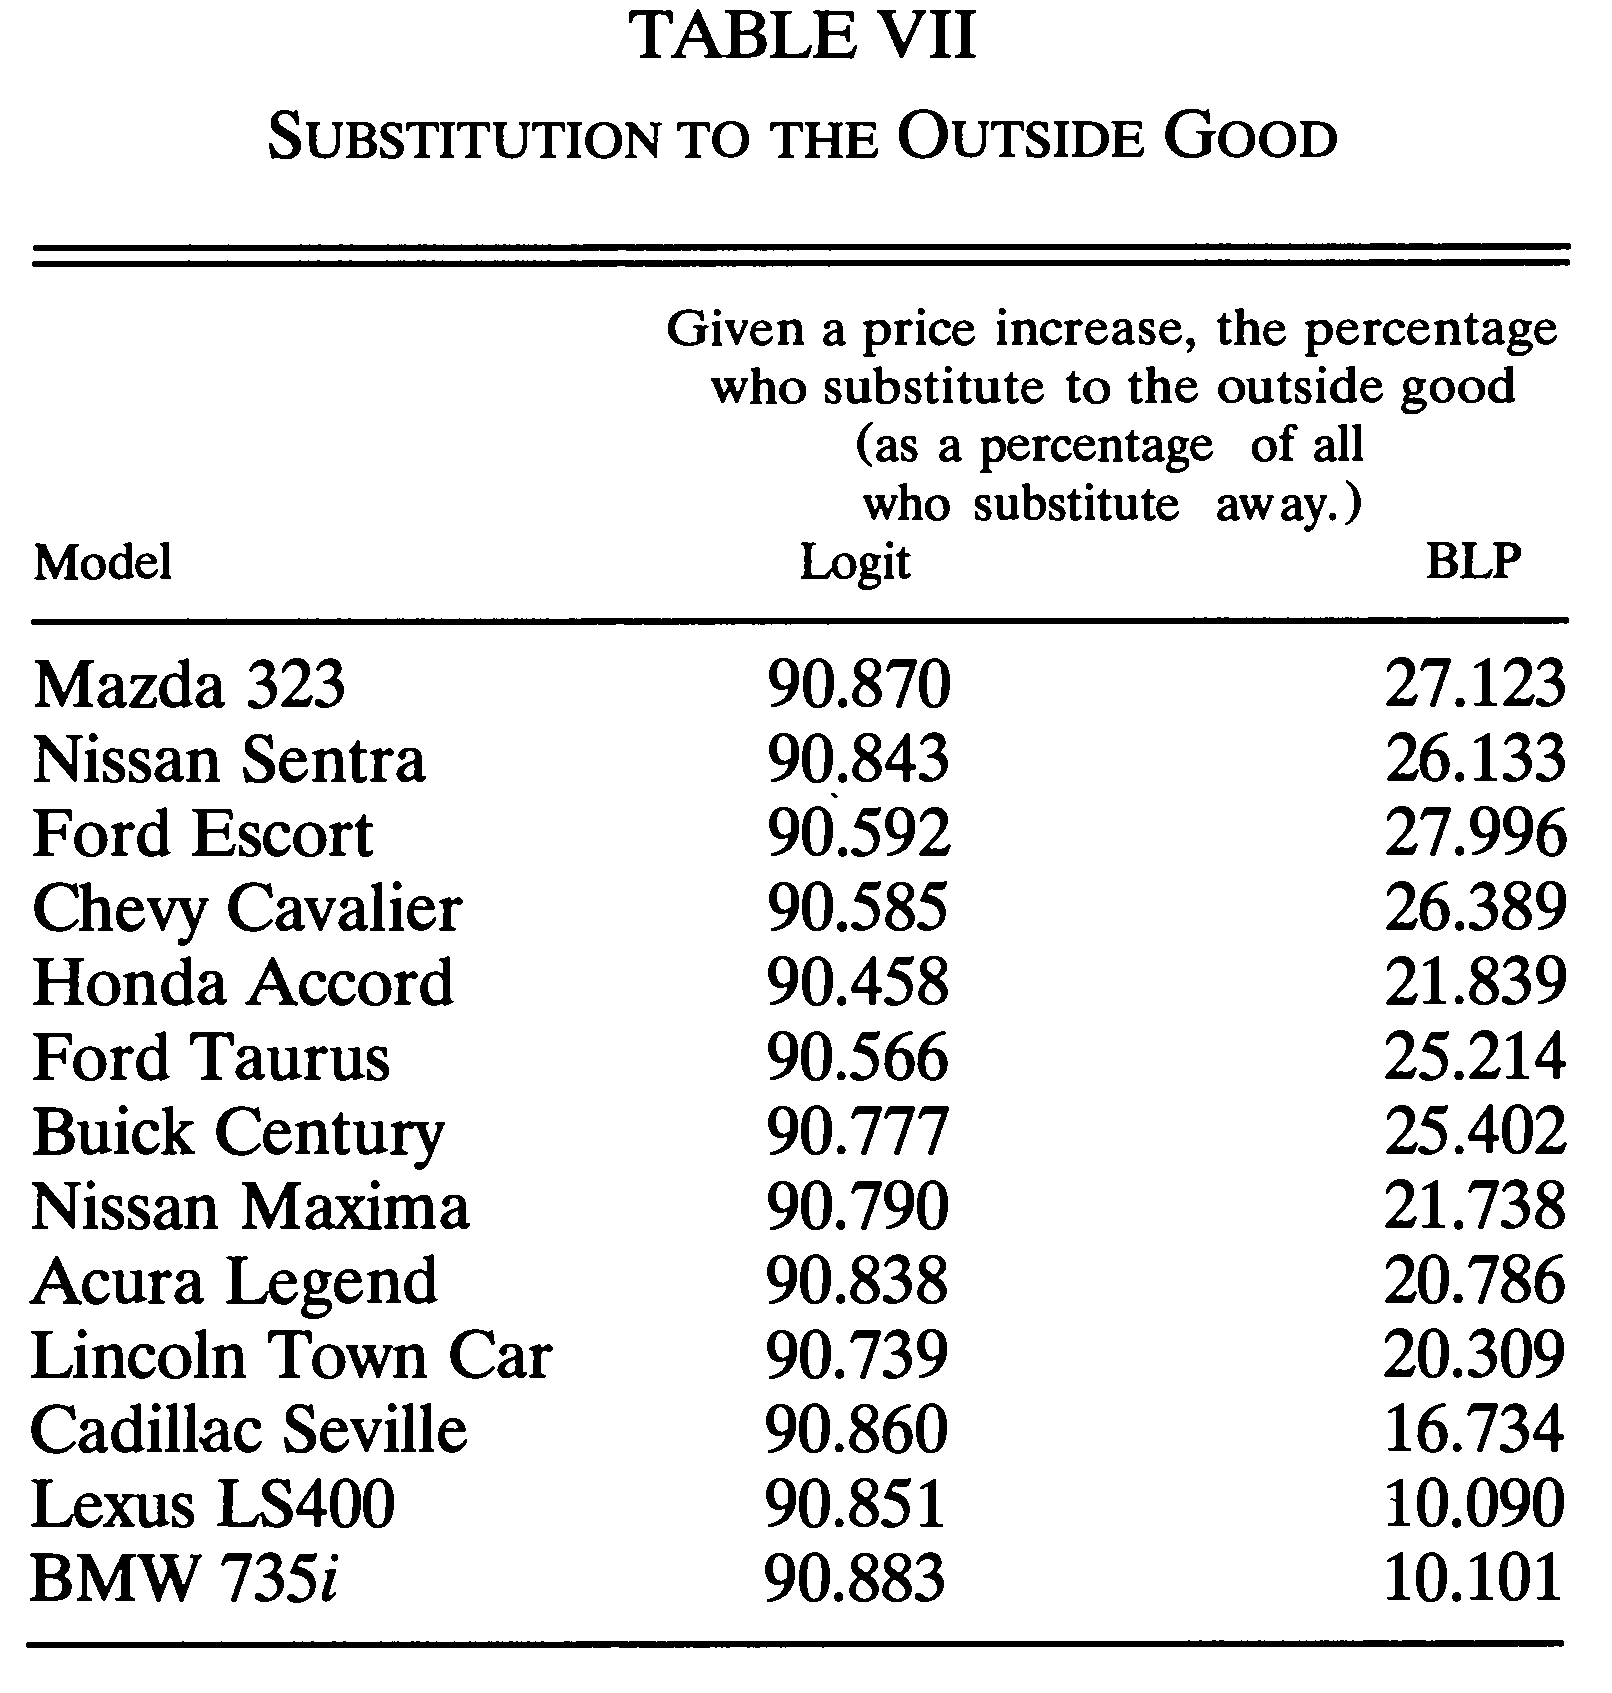
\includegraphics[width=0.6\textwidth]{outside_good.png}
\end{frame}

\begin{frame}\frametitle{Markups}
    \centering
    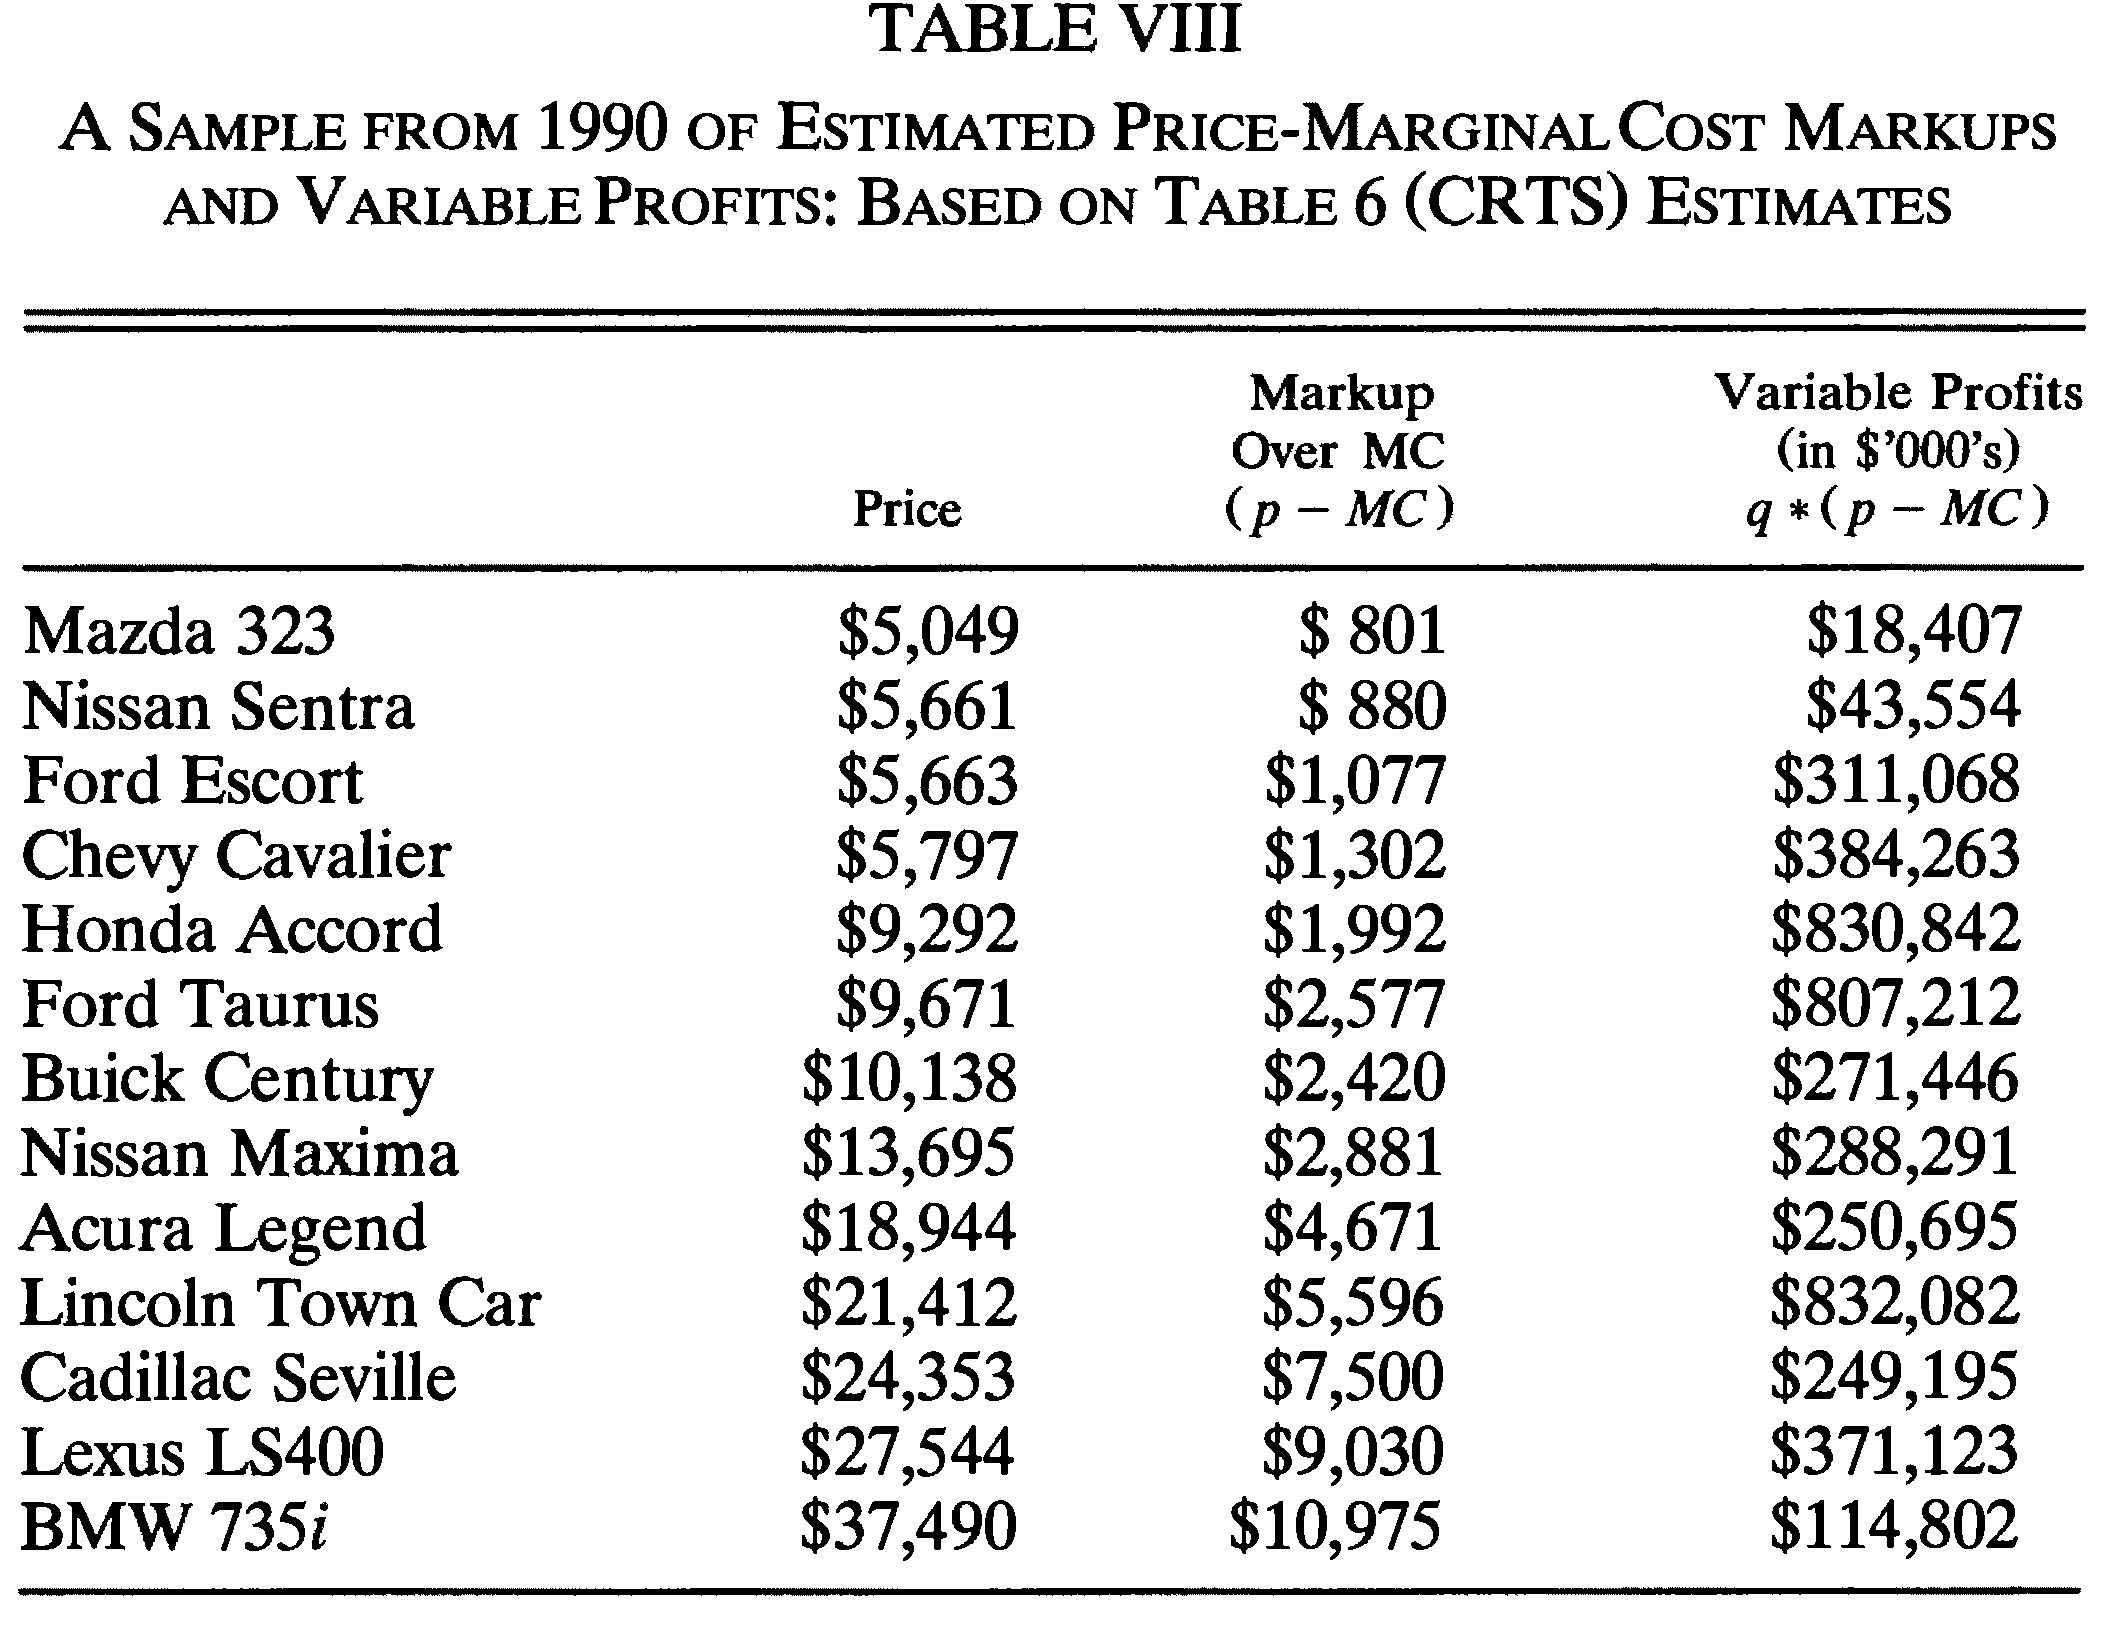
\includegraphics[width=0.8\textwidth]{markups.png}
\end{frame}

\begin{frame}\frametitle{Announcements}
    Office hours
    \begin{itemize}
        \item Reminder: 2:00--3:00 on Tuesdays in 218 Stockbridge
    \end{itemize}
    \vspace{3ex}
    Upcoming
    \begin{itemize}
        \item Final exam is posted, due December 19
        \item Course surveys are open, due December 22
        \begin{itemize}
            \item \href{http://owl.umass.edu/partners/courseEvalSurvey/uma/}{Click here (\texttt{owl.umass.edu/partners/courseEvalSurvey/uma})}
        \end{itemize}
    \end{itemize}
\end{frame}

\end{document}